\subsubsection{Simulation of the $x_I$ and $y_I$ Controllers}
The final design for the $x_I$ and $y_I$ translational controllers is simulated in the following. The simulations are both of the translational velocity controller and the positioning controller. Simulations of the controllers subjected to a step input reference signal and a corresponding simulation showing the related control action of each controller is presented. 


In \autoref{fig:velocityControllersXY} the translational velocity controllers, $\dot{x}_I$ and $\dot{y}_I$, is subjected to a step input reference signal of \SI{1}{m s^{-1}} at $0.5$ \si{s} and $2.5$ \si{s}. This yields a settling time of ?? and an overshoot of ??. 

\begin{minipage}{\linewidth}
    \begin{minipage}{0.5\linewidth}
        \begin{figure}[H]
            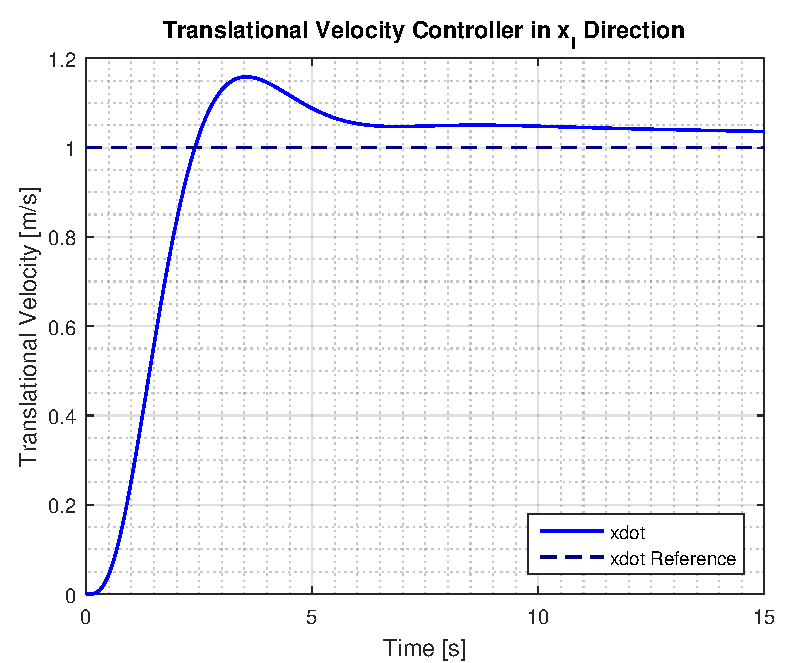
\includegraphics[scale=.58]{figures/velocityControllersXY}
            \centering			
            \captionof{figure}{A step response of the translational velocity controllers in $\dot{x}_I$ and $\dot{y}_I$. Both $\dot{x}_I$ and $\dot{y}_I$ is subjected to a step input reference signal of \SI{1}{m s^{-1}}. $\dot{x}_I$ at $0.5$ \si{s} and $y_I$ at $2.5$ \si{s}.}
            \label{fig:velocityControllersXY}
        \end{figure}
    \end{minipage}
    \hspace{0.03\linewidth}
    \begin{minipage}{0.5\linewidth}
        \begin{figure}[H]
            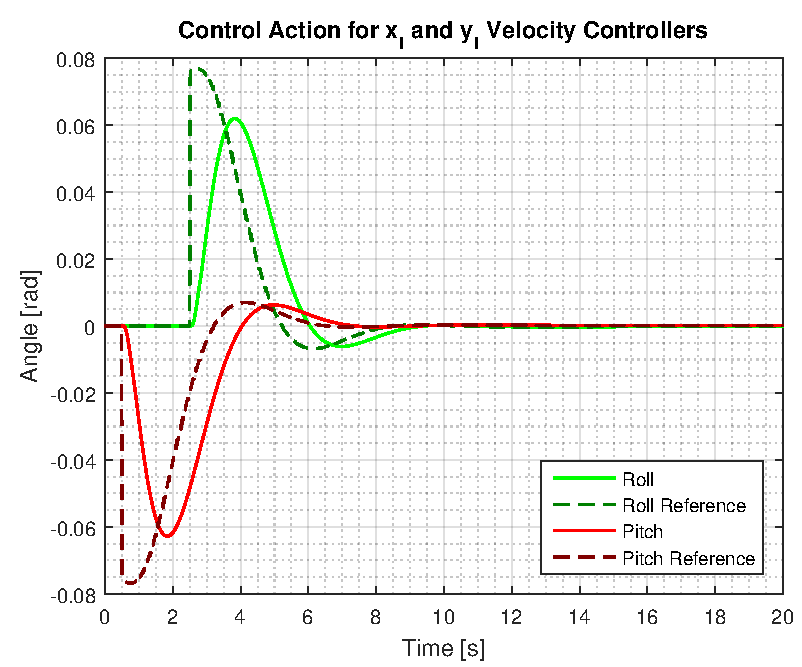
\includegraphics[scale=.58]{figures/velocityControllersXYAction}
            \centering
            \captionof{figure}{The actual control action for the actual performed step input together with the required control action needed to achieve the set step input from \autoref{fig:velocityControllersXY}.}
            \label{fig:velocityControllersXYAction}
        \end{figure}
    \end{minipage}
\end{minipage}

In \autoref{fig:positionControllersXY} the translational velocity controllers, $x_I$ and $y_I$, is subjected to a step input reference signal of \SI{1}{m s^{-1}} at $0.5$ \si{s} and $2.5$ \si{s}. Yielding a settling time of ?? and a overshoot of ??.

\begin{minipage}{\linewidth}
    \begin{minipage}{0.46\linewidth}
        \begin{figure}[H]
            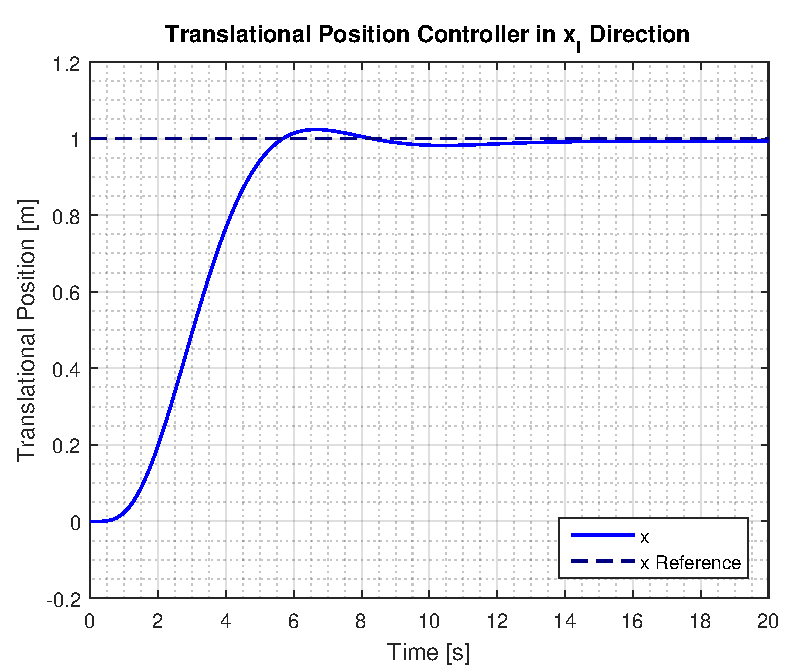
\includegraphics[scale=.61]{figures/positionControllersXY}
            \centering			
            \captionof{figure}{A step response of the position controllers in $x_I$ and $y_I$. Both $x_I$ and $y_I$ is subjected to a step input reference signal of \SI{1}{m s^{-1}}. $x_I$ at $0.5$ \si{s} and $y_I$ at $2.5$ \si{s}.}
            \label{fig:positionControllersXY}
        \end{figure}
    \end{minipage}
    \hspace{0.03\linewidth}
    \begin{minipage}{0.46\linewidth}
        \begin{figure}[H]
            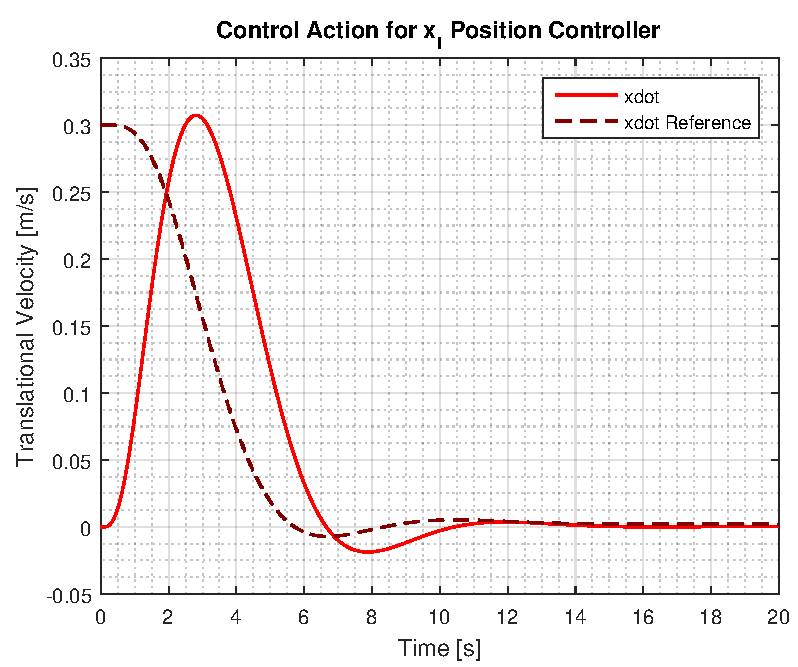
\includegraphics[scale=.61]{figures/positionControllersXYAction}
            \centering
            \captionof{figure}{The actual control action for the actual performed step  together with the required control action needed to achieve the set step reference from \autoref{fig:positionControllersXY}.}
            \label{fig:positionControllersXYAction}
        \end{figure}
    \end{minipage}
\end{minipage}

